% mnras_template.tex
%
% LaTeX template for creating an MNRAS paper
%
% v3.0 released 14 May 2015
% (version numbers match those of mnras.cls)
%
% Copyright (C) Royal Astronomical Society 2015
% Authors:
% Keith T. Smith (Royal Astronomical Society)

% Change log
%
% v3.0 May 2015
%    Renamed to match the new package name
%    Version number matches mnras.cls
%    A few minor tweaks to wording
% v1.0 September 2013
%    Beta testing only - never publicly released
%    First version: a simple (ish) template for creating an MNRAS paper

%%%%%%%%%%%%%%%%%%%%%%%%%%%%%%%%%%%%%%%%%%%%%%%%%%
% Basic setup. Most papers should leave these options alone.
\documentclass[a4paper,fleqn,usenatbib]{mnras}

% MNRAS is set in Times font. If you don't have this installed (most LaTeX
% installations will be fine) or prefer the old Computer Modern fonts, comment
% out the following line
\usepackage{newtxtext,newtxmath}
% Depending on your LaTeX fonts installation, you might get better results with one of these:
%\usepackage{mathptmx}
%\usepackage{txfonts}

% Use vector fonts, so it zooms properly in on-screen viewing software
% Don't change these lines unless you know what you are doing
\usepackage[T1]{fontenc}
\usepackage{ae,aecompl}





\usepackage{graphicx}
\usepackage{subcaption}
\usepackage{float}

\usepackage{color}
\usepackage{booktabs,chemformula}
\usepackage[export]{adjustbox}


\usepackage{tabularx}

\usepackage{caption}
\usepackage{subcaption}
\usepackage{amsmath}

\usepackage{tikz}
\usepackage{hyperref}


%%%%%%%%%%%%%%%%%%% TITLE PAGE %%%%%%%%%%%%%%%%%%%

% Title of the paper, and the short title which is used in the headers.
% Keep the title short and informative.
\title[Short title, max. 45 characters]{Mg Depleted and K Enriched Stars from LAMOST Spectral Data}

% The list of authors, and the short list which is used in the headers.
% If you need two or more lines of authors, add an extra line using \newauthor
\author[Kemp et al.]{
Alex J. Kemp,$^{1}$\thanks{E-mail: ajkem1@student.monash.edu}
A. N. Other,$^{2}$
Third Author$^{2,3}$
and Fourth Author$^{3}$
\\
% List of institutions
$^{1}$Royal Astronomical Society, Burlington House, Piccadilly, London W1J 0BQ, UK\\
$^{2}$Department, Institution, Street Address, City Postal Code, Country\\
$^{3}$Another Department, Different Institution, Street Address, City Postal Code, Country
}

% These dates will be filled out by the publisher
\date{Accepted XXX. Received YYY; in original form ZZZ}

% Enter the current year, for the copyright statements etc.
\pubyear{2015}


\begin{document}
\label{firstpage}
\pagerange{\pageref{firstpage}--\pageref{lastpage}}
\maketitle

% Abstract of the paper
\begin{abstract}

\end{abstract}

% Select between one and six entries from the list of approved keywords.
% Don't make up new ones.
\begin{keywords}
keyword1 -- keyword2 -- keyword3
\end{keywords}

%%%%%%%%%%%%%%%%%%%%%%%%%%%%%%%%%%%%%%%%%%%%%%%%%%

%%%%%%%%%%%%%%%%% BODY OF PAPER %%%%%%%%%%%%%%%%%%

\section{Introduction}

NGC 2419 is the Milky Way's third most massive cluster, and one of the oldest at an age of 12.3 +/- 1.3 Gy (CITE FORBES AND BRIDGES 2010). It resides in the outer halo 87.5 kpc (original source unknown) from the galactic centre, and has been identified as perhaps one of the most unusual clusters in the galaxy.

A spectroscopic study of RGB giant stars in NGC 2419 led to the discovery discovery of a strong anti-correlation between Mg and K in around 30-40 \% of the studied stars, along with weaker relations in Si, Sc, Ca, Ti and V (CITE MUCIARELLI AND COHEN AND KIRBY 2012). Depletions of Mg within globular clusters are not uncommon, but they are always accompanied with an increase in [Fe/H], with the mechanism for this phenomena being the introduction of $\alpha$ element poor but iron rich material released from Type Ia supernovae locally polluting the 'normal' [Mg/Fe] material released from Type II supernovae. However, the two sub-populations are indistinguishable in their [Fe/H] abundance (Cite Kirby and Cohen), and this mechanism fails to account for the enhanced K abundance or trends in the other elements. 

Recently (cite Young Wook Lee 2017) used a Ca filter to identify two population in NGC 2419 corresponding to two generations of stars: G1, first generation metal poor stars, and G2, second generation stars displaying enhanced Ca and significantly increased He abundance ($\Delta Y = 0.19$). The Mg depleted population identified previously was found to be contained with the G2 population.

With the exception of NGC 2808, where several K enhanced (with weaker enhancements than NGC2419) have been found (cite Muciarelli 2015), this anti-correlation between Mg and K has, with the exception of this study, been found to be contained within NGC 2419, with a targeted search looking at the K abundance in RGB stars from clusters NGC 6752, NGC 6121, NGC 1904, and ω Cen as well as some field stars finding in all cases K abundances falling within the range of the Mg normal population in NGC 2419 (cite carreta 2013).

At present, there is no accepted nuclear process that can explain the elemental abundance in NGC 2419. Although the fact that Mg-K anti-correlation is confined to this specific globular cluster would seem to imply either a small population  of unusual polluter stars of some sort, or a single extremely massive polluter star, the details of these polluter candidates remain unknown.

An early modelling attempt at replicating the anomalous abundances in NGC 2419 assumed hot-bottom burning in AGB and super-AGB stars, with high temperatures of approximately 150 MK, was able to reproduce the Mg-K anti-correlation, through proton capture on Argon, but only if the reaction cross section was set to 100 times the standard rate or temperatures could be made higher than currently accepted values [cite VENTURA 2012]. 

A more recent, comprehensive attempt to replicate not only the Mg and K abundances in NGC 2419 but also the abundances of Si, Sc, Ca, Ti and V, with the aim of constraining the temperatures and pressures required was undertaken by [Cite Illiadis]. It was found that (with the exception of extremely high densities $\>10^8$ g/cm$^3$) temperatures between 100 and 200 MK and densities between 10$^-4$ and 10$^8$ g/cm$^3$. Using this information, core and shell burning of low mass, high mass and super massive stars were ruled out as potential poluter candidates, as well as regular AGB stars. Super-AGB (SAGB) stars however were regarded as potential candidates, with only a relatively small (roughly 10-20 MK) increase in temperature required to fall in the acceptable band of parameter space identified. The other potential candidate identified was Novae, although the lack of detailed models of white dwarfs accreting material similar to NGC 2419 either from a binary companion or the intra cluster medium limit appraisals of its feasibility regarding whether enough ejecta could be produced and retained by the cluster. Estimates based on current novae frequency in globular clusters by [CITE HENZE 2013] carried out in the work conclude that the amount of material that would be produced by Novae is at most 1 \% of the total required mass to pollute 30 \% of NGC 2419.

However, the question remains: why is this signature unique to 2419? It has been suggested that the cluster's position and size, being both very massive and very distant from the Milky Way for a globular cluster, aids it in retaining material from explosive events. This would cause in its first generation polluter stars to have an increased effect on the second generation of stars. It has also been proposed that NGC 2419 is the stripped core of a dwarf spheroidal galaxy similar to $\omega$ Centauri, which would imply that in the past it was even more massive, allowing it to retain its ejecta even more efficiently.

Although to the knowledge of the author not formally studied in terms of feasibility, another suggested polluter candidate is a pair instability super nova (PISN) (CITE CARRETA 2013). Unique to extremely massive population III stars, these events involve the total destruction of the star, with no black hole remnant being left behind. The main argument for this idea is that the extreme rarity of these events, coupled with the huge masses of processed material involved, could perhaps allow the entire signature in NGC 2419 to be the result of a single event, explaining why it is not seen in any other globular clusters.

This study, which queries 450000ish LAMOST giants for depleted Mg and enhanced K, seeks to provide additional data points from which theories regarding the origin of this signature can be developed. 190 strong candidates for this signature, almost all of them not at this time associated with any globular cluster, are detailed in Table [REFERENCE TABLE HERE]. These stars occur at a wide range of metalicities, including solar metalicity. The implications for theories attempting to explain the origin of this signiature first found in NGC 2419 is likely to be significant, as for such a theory to be complete, it must now account not only for the stars in the metal poor NGC 2419, but also these stars existing at a range of metalicities in the galactic plane. Further, the task of explaining the uniqueness of NGC 2419 is not removed, as it remains the only globular cluster to significantly display this phenomena.

\section{Methods, Observations, Simulations etc.}

\textit{The Cannon}, a data based spectral model devloped by \cite{ho2017} using APOGEE data, was fitted to each star in our 450000 star sample of LAMOST giants.
%Ho2017 says that using Appogee, they found almost 10000 giants which were common between the lamost and apoggeee surveys and used that to fit a predictive model to to lamost giants (450000) to determine the 'Teff, logg, [Fe/H], and [α/M]'.
This model is treated as representative of the expected spectra for each star.

The residuals were taken of the normalised LAMOST flux data and 
\textit{The Cannon} according to $residual=data-model$. A positive residual implies a higher normalised flux than expected by the model, while a negative residual implies a lower normalised flux than expected. In turn, at a given spectral line a lower normalised flux is associated with an over-abundance, while a higher normalised flux is associated with a depleted abundance.

A Gaussian curve was fitted to the residuals about each spectral line in the Mg triplet (5167 \AA, 5172 \AA, 5184 \AA) as well as the K doublet (7665 \AA, 7699 \AA) to characterise any deviation from the model. The amplitude and amplitude error for this curve was then used as the basis for a data filter designed to produce potential candidate stars with spectra indicative of Mg depletion, as well as K enrichment.

Two filters were applied separately, with the candidate pool formed from all unique stars identified in either filter. The first, broader filter required the Mg 5184 line's Gaussian to satisfy $Amp > 0.05$ and $\frac{Amp}{Amp_{err}}>3$, and the K 7665 line to satisfy $Amp < 0.05$ and $\frac{Amp}{Amp_{err}}>3$. The second, more demanding filter was applied to require 2 of the three Mg lines to satisfy $Amp > 0.05$ and $\frac{Amp}{Amp_{err}}>3$, as well as either of the K lines. These filters together produced 280 candidate stars to be vetted manually.

The vetting process was done through visual examination of each case. The minimum criterion for a pass was two out of the three Mg lines to look at least plausibly depleted, and at least one of the K lines to look convincing. The local noisiness of the signal was taken into account when making these determinations. Of the 280 candidates manually vetted, 156 were ultimately determined to be sufficiently strong candidates to make the list, presented in Table [INSERT TABLE REFERENCE HERE].

\subsection{Figures and tables}

Figures and tables should be placed at logical positions in the text. Don't
worry about the exact layout, which will be handled by the publishers.

Figures are referred to as e.g. Fig.~\ref{fig:example_figure}, and tables as
e.g. Table~\ref{tab:example_table}.




\begin{figure}
\centering
\begin{subfigure}{.5\linewidth}
  \centering
  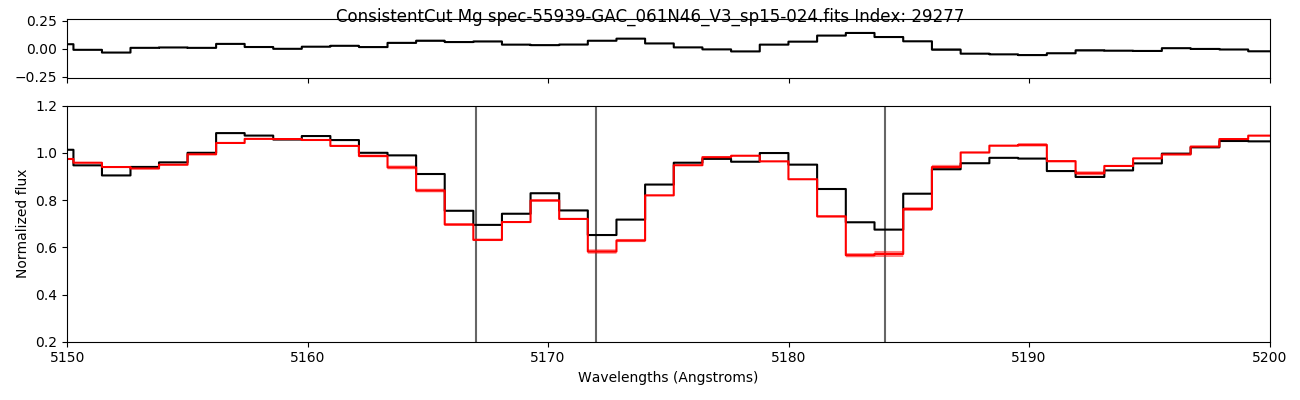
\includegraphics[width=.95\linewidth]{29277_Mg}
  \caption{Mg}
  \label{Mgposter}
\end{subfigure}%       %Note: the % to the left is VERY IMPORTANT.

\begin{subfigure}{.5\linewidth}
  \centering
  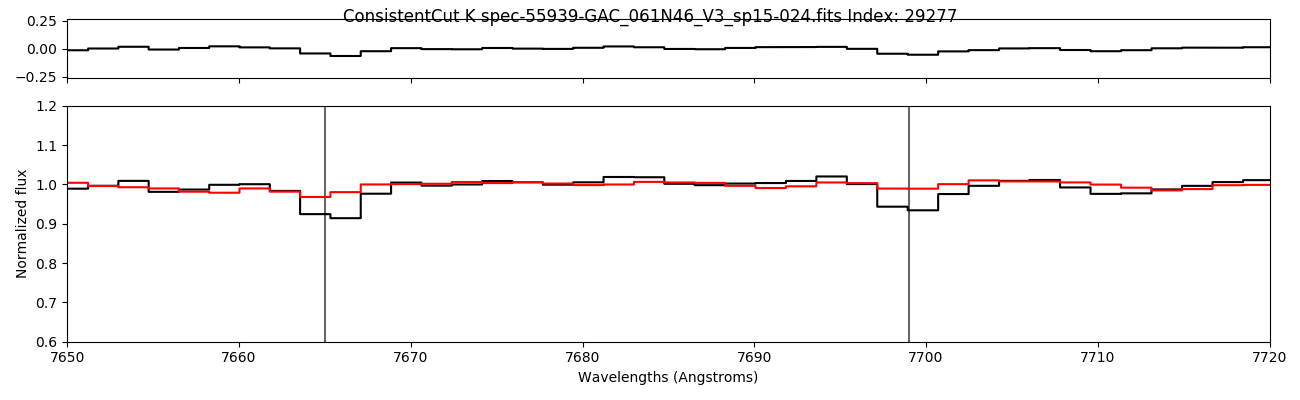
\includegraphics[width=.95\linewidth]{29277_K}
  \caption{K}
  \label{Kposter}
\end{subfigure}
\caption{}
\label{posterchildren}
\end{figure} 

\begin{figure}
	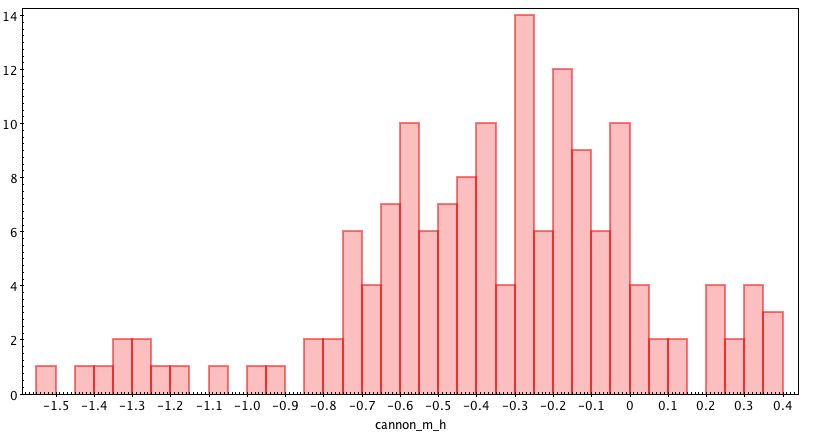
\includegraphics[width=\columnwidth]{m_hhist.png}
    \caption{Metalicity Histogram}
    \label{mhist}
\end{figure}


\begin{figure}
	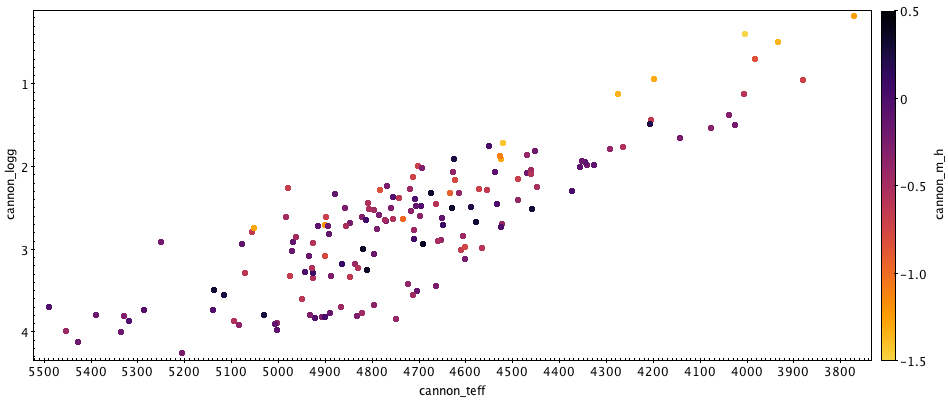
\includegraphics[width=\columnwidth]{teff_logg.png}
    \caption{Effective temperature, log surface gravity, metalicity}
    \label{mhist}
\end{figure}

\begin{figure}
	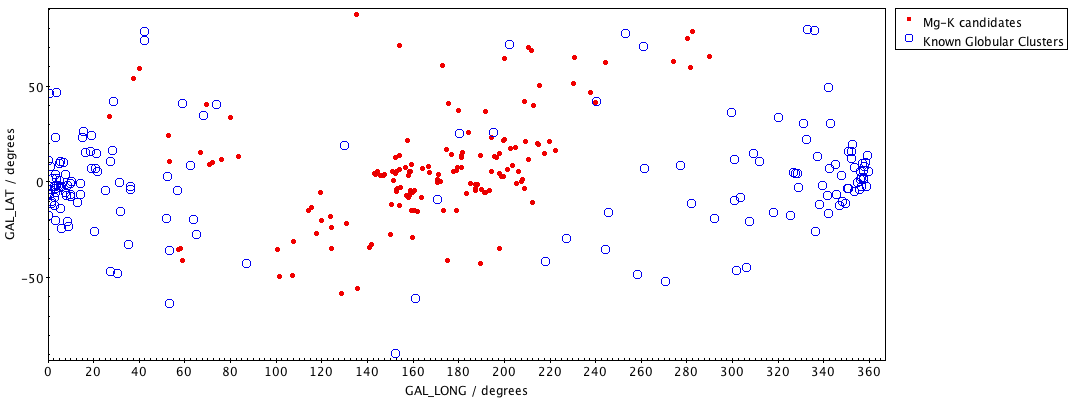
\includegraphics[width=\columnwidth]{galcoord.png}
    \caption{Galactic coordinates for Mg-K stars and known globular clusters}
    \label{mhist}
\end{figure}

% Example table
\begin{table}
	\centering
	\caption{This is an example table. Captions appear above each table.
	Remember to define the quantities, symbols and units used.}
	\label{tab:example_table}
	\begin{tabular}{lccr} % four columns, alignment for each
		\hline
		A & B & C & D\\
		\hline
		1 & 2 & 3 & 4\\
		2 & 4 & 6 & 8\\
		3 & 5 & 7 & 9\\
		\hline
	\end{tabular}
\end{table}


\section{Conclusions}

The last numbered section should briefly summarise what has been done, and describe
the final conclusions which the authors draw from their work.

\section*{Acknowledgements}

The Acknowledgements section is not numbered. Here you can thank helpful
colleagues, acknowledge funding agencies, telescopes and facilities used etc.
Try to keep it short.

%%%%%%%%%%%%%%%%%%%%%%%%%%%%%%%%%%%%%%%%%%%%%%%%%%

%%%%%%%%%%%%%%%%%%%% REFERENCES %%%%%%%%%%%%%%%%%%

% The best way to enter references is to use BibTeX:

\bibliographystyle{mnras}
\bibliography{mgkbib} % if your bibtex file is called example.bib


% Alternatively you could enter them by hand, like this:
% This method is tedious and prone to error if you have lots of references


%%%%%%%%%%%%%%%%%%%%%%%%%%%%%%%%%%%%%%%%%%%%%%%%%%

%%%%%%%%%%%%%%%%% APPENDICES %%%%%%%%%%%%%%%%%%%%%

\appendix

\section{Some extra material}

If you want to present additional material which would interrupt the flow of the main paper,
it can be placed in an Appendix which appears after the list of references.

%%%%%%%%%%%%%%%%%%%%%%%%%%%%%%%%%%%%%%%%%%%%%%%%%%


% Don't change these lines
\bsp	% typesetting comment
\label{lastpage}
\end{document}

% End of mnras_template.tex